\documentclass[1p]{elsarticle_modified}
%\bibliographystyle{elsarticle-num}

%\usepackage[colorlinks]{hyperref}
%\usepackage{abbrmath_seonhwa} %\Abb, \Ascr, \Acal ,\Abf, \Afrak
\usepackage{amsfonts}
\usepackage{amssymb}
\usepackage{amsmath}
\usepackage{amsthm}
\usepackage{scalefnt}
\usepackage{amsbsy}
\usepackage{kotex}
\usepackage{caption}
\usepackage{subfig}
\usepackage{color}
\usepackage{graphicx}
\usepackage{xcolor} %% white, black, red, green, blue, cyan, magenta, yellow
\usepackage{float}
\usepackage{setspace}
\usepackage{hyperref}

\usepackage{tikz}
\usetikzlibrary{arrows}

\usepackage{multirow}
\usepackage{array} % fixed length table
\usepackage{hhline}

%%%%%%%%%%%%%%%%%%%%%
\makeatletter
\renewcommand*\env@matrix[1][\arraystretch]{%
	\edef\arraystretch{#1}%
	\hskip -\arraycolsep
	\let\@ifnextchar\new@ifnextchar
	\array{*\c@MaxMatrixCols c}}
\makeatother %https://tex.stackexchange.com/questions/14071/how-can-i-increase-the-line-spacing-in-a-matrix
%%%%%%%%%%%%%%%

\usepackage[normalem]{ulem}

\newcommand{\msout}[1]{\ifmmode\text{\sout{\ensuremath{#1}}}\else\sout{#1}\fi}
%SOURCE: \msout is \stkout macro in https://tex.stackexchange.com/questions/20609/strikeout-in-math-mode

\newcommand{\cancel}[1]{
	\ifmmode
	{\color{red}\msout{#1}}
	\else
	{\color{red}\sout{#1}}
	\fi
}

\newcommand{\add}[1]{
	{\color{blue}\uwave{#1}}
}

\newcommand{\replace}[2]{
	\ifmmode
	{\color{red}\msout{#1}}{\color{blue}\uwave{#2}}
	\else
	{\color{red}\sout{#1}}{\color{blue}\uwave{#2}}
	\fi
}

\newcommand{\Sol}{\mathcal{S}} %segment
\newcommand{\D}{D} %diagram
\newcommand{\A}{\mathcal{A}} %arc


%%%%%%%%%%%%%%%%%%%%%%%%%%%%%5 test

\def\sl{\operatorname{\textup{SL}}(2,\Cbb)}
\def\psl{\operatorname{\textup{PSL}}(2,\Cbb)}
\def\quan{\mkern 1mu \triangleright \mkern 1mu}

\theoremstyle{definition}
\newtheorem{thm}{Theorem}[section]
\newtheorem{prop}[thm]{Proposition}
\newtheorem{lem}[thm]{Lemma}
\newtheorem{ques}[thm]{Question}
\newtheorem{cor}[thm]{Corollary}
\newtheorem{defn}[thm]{Definition}
\newtheorem{exam}[thm]{Example}
\newtheorem{rmk}[thm]{Remark}
\newtheorem{alg}[thm]{Algorithm}

\newcommand{\I}{\sqrt{-1}}
\begin{document}

%\begin{frontmatter}
%
%\title{Boundary parabolic representations of knots up to 8 crossings}
%
%%% Group authors per affiliation:
%\author{Yunhi Cho} 
%\address{Department of Mathematics, University of Seoul, Seoul, Korea}
%\ead{yhcho@uos.ac.kr}
%
%
%\author{Seonhwa Kim} %\fnref{s_kim}}
%\address{Center for Geometry and Physics, Institute for Basic Science, Pohang, 37673, Korea}
%\ead{ryeona17@ibs.re.kr}
%
%\author{Hyuk Kim}
%\address{Department of Mathematical Sciences, Seoul National University, Seoul 08826, Korea}
%\ead{hyukkim@snu.ac.kr}
%
%\author{Seokbeom Yoon}
%\address{Department of Mathematical Sciences, Seoul National University, Seoul, 08826,  Korea}
%\ead{sbyoon15@snu.ac.kr}
%
%\begin{abstract}
%We find all boundary parabolic representation of knots up to 8 crossings.
%
%\end{abstract}
%\begin{keyword}
%    \MSC[2010] 57M25 
%\end{keyword}
%
%\end{frontmatter}

%\linenumbers
%\tableofcontents
%
\newcommand\colored[1]{\textcolor{white}{\rule[-0.35ex]{0.8em}{1.4ex}}\kern-0.8em\color{red} #1}%
%\newcommand\colored[1]{\textcolor{white}{ #1}\kern-2.17ex	\textcolor{white}{ #1}\kern-1.81ex	\textcolor{white}{ #1}\kern-2.15ex\color{red}#1	}

{\Large $\underline{11a_{53}~(K11a_{53})}$}

\setlength{\tabcolsep}{10pt}
\renewcommand{\arraystretch}{1.6}
\vspace{1cm}\begin{tabular}{m{100pt}>{\centering\arraybackslash}m{274pt}}
\multirow{5}{120pt}{
	\centering
	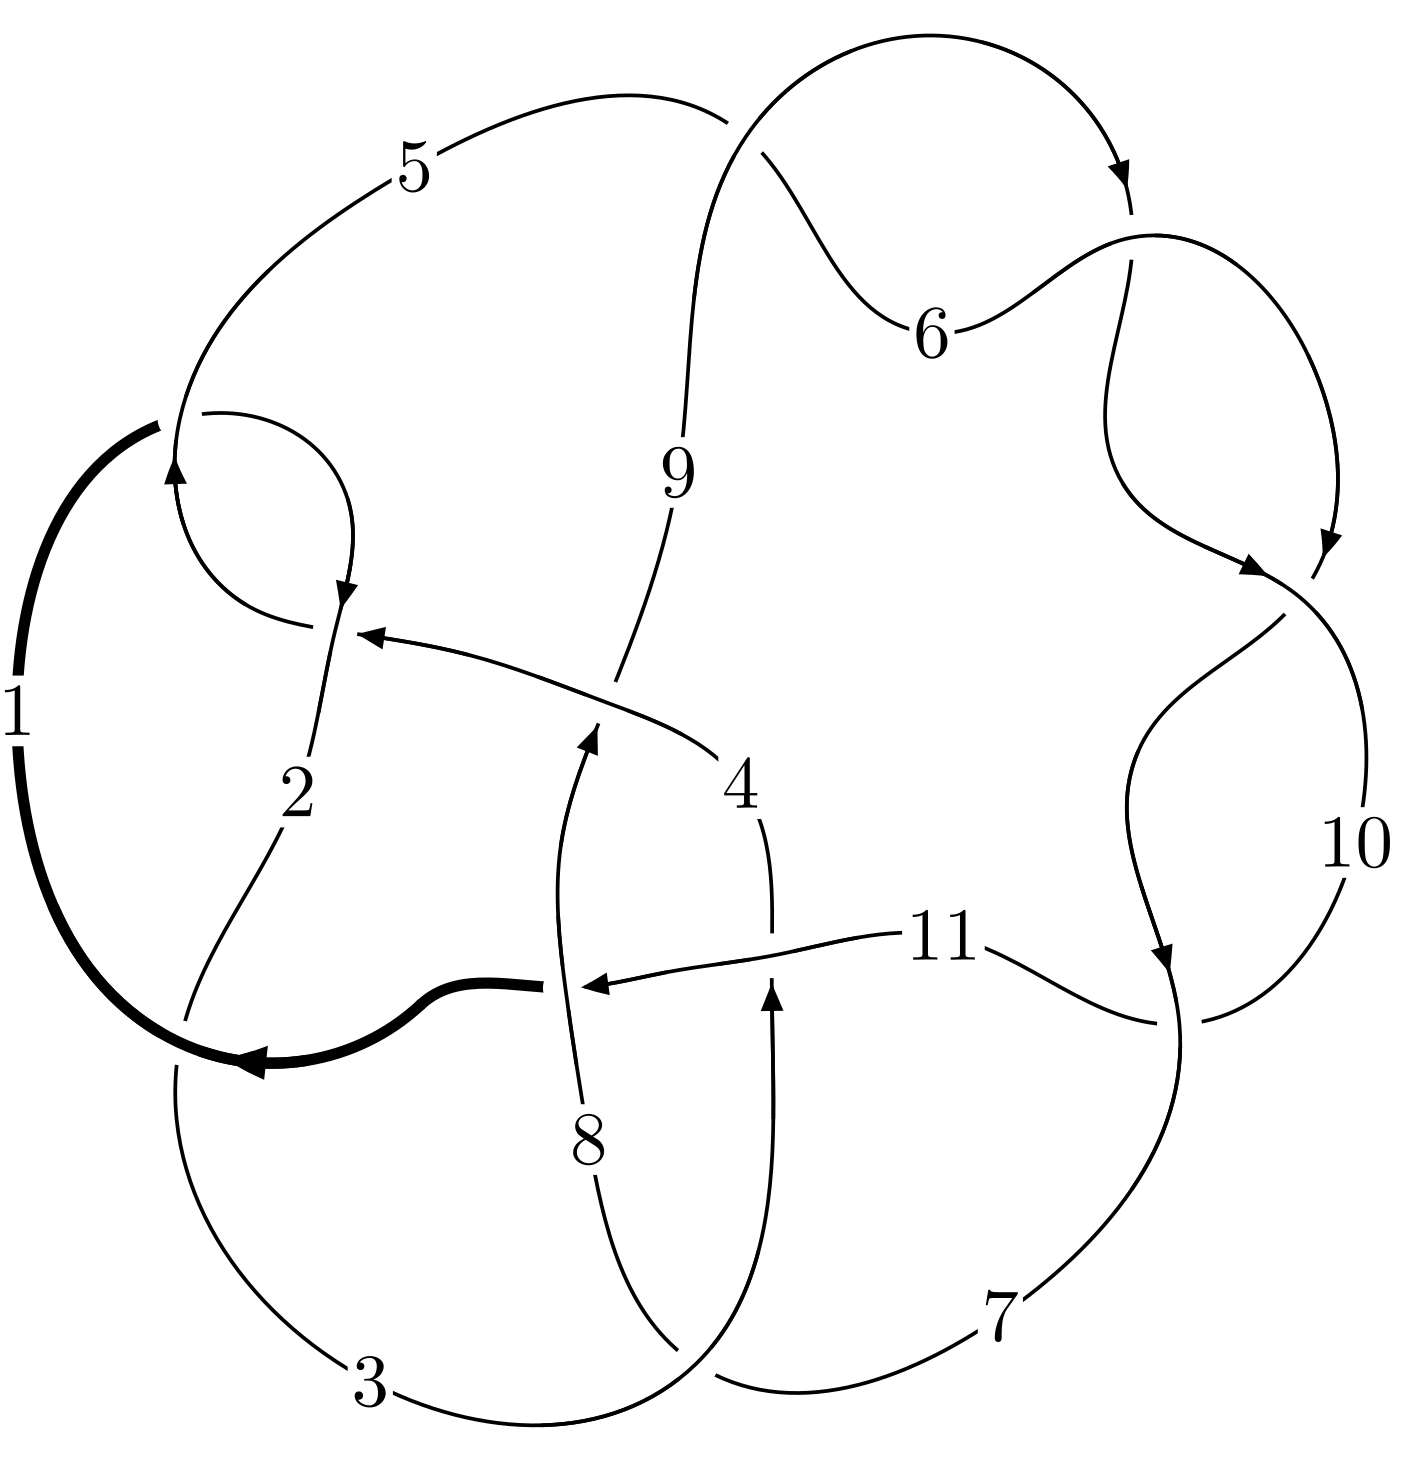
\includegraphics[width=112pt]{../../../GIT/diagram.site/Diagrams/png/302_11a_53.png}\\
\ \ \ A knot diagram\footnotemark}&
\allowdisplaybreaks
\textbf{Linearized knot diagam} \\
\cline{2-2}
 &
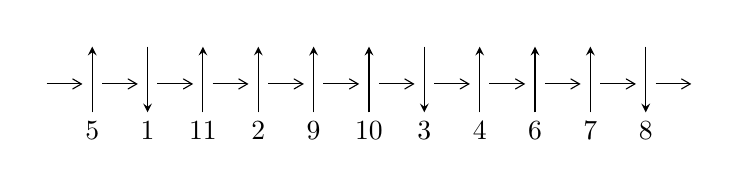
\begin{tikzpicture}[x=20pt, y=17pt]
	% nodes
	\node (C0) at (0, 0) {};
	\node (C1) at (1, 0) {};
	\node (C1U) at (1, +1) {};
	\node (C1D) at (1, -1) {5};

	\node (C2) at (2, 0) {};
	\node (C2U) at (2, +1) {};
	\node (C2D) at (2, -1) {1};

	\node (C3) at (3, 0) {};
	\node (C3U) at (3, +1) {};
	\node (C3D) at (3, -1) {11};

	\node (C4) at (4, 0) {};
	\node (C4U) at (4, +1) {};
	\node (C4D) at (4, -1) {2};

	\node (C5) at (5, 0) {};
	\node (C5U) at (5, +1) {};
	\node (C5D) at (5, -1) {9};

	\node (C6) at (6, 0) {};
	\node (C6U) at (6, +1) {};
	\node (C6D) at (6, -1) {10};

	\node (C7) at (7, 0) {};
	\node (C7U) at (7, +1) {};
	\node (C7D) at (7, -1) {3};

	\node (C8) at (8, 0) {};
	\node (C8U) at (8, +1) {};
	\node (C8D) at (8, -1) {4};

	\node (C9) at (9, 0) {};
	\node (C9U) at (9, +1) {};
	\node (C9D) at (9, -1) {6};

	\node (C10) at (10, 0) {};
	\node (C10U) at (10, +1) {};
	\node (C10D) at (10, -1) {7};

	\node (C11) at (11, 0) {};
	\node (C11U) at (11, +1) {};
	\node (C11D) at (11, -1) {8};
	\node (C12) at (12, 0) {};

	% arrows
	\draw[->,>={angle 60}]
	(C0) edge (C1) (C1) edge (C2) (C2) edge (C3) (C3) edge (C4) (C4) edge (C5) (C5) edge (C6) (C6) edge (C7) (C7) edge (C8) (C8) edge (C9) (C9) edge (C10) (C10) edge (C11) (C11) edge (C12) ;	\draw[->,>=stealth]
	(C1D) edge (C1U) (C2U) edge (C2D) (C3D) edge (C3U) (C4D) edge (C4U) (C5D) edge (C5U) (C6D) edge (C6U) (C7U) edge (C7D) (C8D) edge (C8U) (C9D) edge (C9U) (C10D) edge (C10U) (C11U) edge (C11D) ;
	\end{tikzpicture} \\
\hhline{~~} \\& 
\textbf{Solving Sequence} \\ \cline{2-2} 
 &
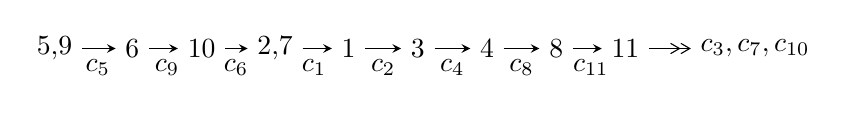
\begin{tikzpicture}[x=25pt, y=7pt]
	% node
	\node (A0) at (-1/8, 0) {5,9};
	\node (A1) at (1, 0) {6};
	\node (A2) at (2, 0) {10};
	\node (A3) at (49/16, 0) {2,7};
	\node (A4) at (33/8, 0) {1};
	\node (A5) at (41/8, 0) {3};
	\node (A6) at (49/8, 0) {4};
	\node (A7) at (57/8, 0) {8};
	\node (A8) at (65/8, 0) {11};
	\node (C1) at (1/2, -1) {$c_{5}$};
	\node (C2) at (3/2, -1) {$c_{9}$};
	\node (C3) at (5/2, -1) {$c_{6}$};
	\node (C4) at (29/8, -1) {$c_{1}$};
	\node (C5) at (37/8, -1) {$c_{2}$};
	\node (C6) at (45/8, -1) {$c_{4}$};
	\node (C7) at (53/8, -1) {$c_{8}$};
	\node (C8) at (61/8, -1) {$c_{11}$};
	\node (A9) at (10, 0) {$c_{3},c_{7},c_{10}$};

	% edge
	\draw[->,>=stealth]	
	(A0) edge (A1) (A1) edge (A2) (A2) edge (A3) (A3) edge (A4) (A4) edge (A5) (A5) edge (A6) (A6) edge (A7) (A7) edge (A8) ;
	\draw[->>,>={angle 60}]	
	(A8) edge (A9);
\end{tikzpicture} \\ 

\end{tabular} \\

\footnotetext{
The image of knot diagram is generated by the software ``\textbf{Draw programme}" developed by Andrew Bartholomew(\url{http://www.layer8.co.uk/maths/draw/index.htm\#Running-draw}), where we modified some parts for our purpose(\url{https://github.com/CATsTAILs/LinksPainter}).
}\phantom \\ \newline 
\centering \textbf{Ideals for irreducible components\footnotemark of $X_{\text{par}}$} 
 
\begin{align*}
I^u_{1}&=\langle 
2.81606\times10^{31} u^{49}+5.08261\times10^{31} u^{48}+\cdots+4.27879\times10^{31} b-1.93634\times10^{30},\\
\phantom{I^u_{1}}&\phantom{= \langle  }-4.15334\times10^{31} u^{49}-1.01081\times10^{32} u^{48}+\cdots+5.34849\times10^{30} a+8.37501\times10^{31},\;u^{50}+3 u^{49}+\cdots-8 u-1\rangle \\
I^u_{2}&=\langle 
b^2- b+1,\;a+1,\;u+1\rangle \\
\\
\end{align*}
\raggedright * 2 irreducible components of $\dim_{\mathbb{C}}=0$, with total 52 representations.\\
\footnotetext{All coefficients of polynomials are rational numbers. But the coefficients are sometimes approximated in decimal forms when there is not enough margin.}
\newpage
\renewcommand{\arraystretch}{1}
\centering \section*{I. $I^u_{1}= \langle 2.82\times10^{31} u^{49}+5.08\times10^{31} u^{48}+\cdots+4.28\times10^{31} b-1.94\times10^{30},\;-4.15\times10^{31} u^{49}-1.01\times10^{32} u^{48}+\cdots+5.35\times10^{30} a+8.38\times10^{31},\;u^{50}+3 u^{49}+\cdots-8 u-1 \rangle$}
\flushleft \textbf{(i) Arc colorings}\\
\begin{tabular}{m{7pt} m{180pt} m{7pt} m{180pt} }
\flushright $a_{5}=$&$\begin{pmatrix}1\\0\end{pmatrix}$ \\
\flushright $a_{9}=$&$\begin{pmatrix}0\\u\end{pmatrix}$ \\
\flushright $a_{6}=$&$\begin{pmatrix}1\\- u^2\end{pmatrix}$ \\
\flushright $a_{10}=$&$\begin{pmatrix}u\\- u^3+u\end{pmatrix}$ \\
\flushright $a_{2}=$&$\begin{pmatrix}7.76545 u^{49}+18.8989 u^{48}+\cdots-81.3213 u-15.6586\\-0.658144 u^{49}-1.18786 u^{48}+\cdots+4.71381 u+0.0452544\end{pmatrix}$ \\
\flushright $a_{7}=$&$\begin{pmatrix}- u^2+1\\u^4-2 u^2\end{pmatrix}$ \\
\flushright $a_{1}=$&$\begin{pmatrix}8.42359 u^{49}+20.0868 u^{48}+\cdots-86.0351 u-15.7039\\-0.658144 u^{49}-1.18786 u^{48}+\cdots+4.71381 u+0.0452544\end{pmatrix}$ \\
\flushright $a_{3}=$&$\begin{pmatrix}16.5522 u^{49}+40.5819 u^{48}+\cdots-183.821 u-29.5368\\-0.186883 u^{49}-0.0491952 u^{48}+\cdots-0.958193 u+0.142958\end{pmatrix}$ \\
\flushright $a_{4}=$&$\begin{pmatrix}-15.7480 u^{49}-38.5171 u^{48}+\cdots+171.517 u+27.4764\\0.344150 u^{49}+0.520346 u^{48}+\cdots-2.34513 u-0.685097\end{pmatrix}$ \\
\flushright $a_{8}=$&$\begin{pmatrix}-13.2353 u^{49}-30.8285 u^{48}+\cdots+140.710 u+20.3271\\3.76331 u^{49}+9.12279 u^{48}+\cdots-33.9045 u-5.65366\end{pmatrix}$ \\
\flushright $a_{11}=$&$\begin{pmatrix}- u^3+2 u\\u^5-3 u^3+u\end{pmatrix}$\\ \flushright $a_{11}=$&$\begin{pmatrix}- u^3+2 u\\u^5-3 u^3+u\end{pmatrix}$\\&\end{tabular}
\flushleft \textbf{(ii) Obstruction class $= -1$}\\~\\
\flushleft \textbf{(iii) Cusp Shapes $= 24.5612 u^{49}+62.4649 u^{48}+\cdots-284.357 u-43.1928$}\\~\\
\newpage\renewcommand{\arraystretch}{1}
\flushleft \textbf{(iv) u-Polynomials at the component}\newline \\
\begin{tabular}{m{50pt}|m{274pt}}
Crossings & \hspace{64pt}u-Polynomials at each crossing \\
\hline $$\begin{aligned}c_{1},c_{4}\end{aligned}$$&$\begin{aligned}
&u^{50}+2 u^{49}+\cdots-11 u+1
\end{aligned}$\\
\hline $$\begin{aligned}c_{2}\end{aligned}$$&$\begin{aligned}
&u^{50}+18 u^{49}+\cdots-71 u+1
\end{aligned}$\\
\hline $$\begin{aligned}c_{3}\end{aligned}$$&$\begin{aligned}
&u^{50}+5 u^{49}+\cdots+12 u+4
\end{aligned}$\\
\hline $$\begin{aligned}c_{5},c_{6},c_{9}\\c_{10}\end{aligned}$$&$\begin{aligned}
&u^{50}-3 u^{49}+\cdots+8 u-1
\end{aligned}$\\
\hline $$\begin{aligned}c_{7}\end{aligned}$$&$\begin{aligned}
&u^{50}-2 u^{49}+\cdots-293 u-41
\end{aligned}$\\
\hline $$\begin{aligned}c_{8}\end{aligned}$$&$\begin{aligned}
&u^{50}+13 u^{48}+\cdots+3545 u-3881
\end{aligned}$\\
\hline $$\begin{aligned}c_{11}\end{aligned}$$&$\begin{aligned}
&u^{50}+3 u^{49}+\cdots-2 u-1
\end{aligned}$\\
\hline
\end{tabular}\\~\\
\newpage\renewcommand{\arraystretch}{1}
\flushleft \textbf{(v) Riley Polynomials at the component}\newline \\
\begin{tabular}{m{50pt}|m{274pt}}
Crossings & \hspace{64pt}Riley Polynomials at each crossing \\
\hline $$\begin{aligned}c_{1},c_{4}\end{aligned}$$&$\begin{aligned}
&y^{50}+18 y^{49}+\cdots-71 y+1
\end{aligned}$\\
\hline $$\begin{aligned}c_{2}\end{aligned}$$&$\begin{aligned}
&y^{50}+30 y^{49}+\cdots-6727 y+1
\end{aligned}$\\
\hline $$\begin{aligned}c_{3}\end{aligned}$$&$\begin{aligned}
&y^{50}-15 y^{49}+\cdots+24 y+16
\end{aligned}$\\
\hline $$\begin{aligned}c_{5},c_{6},c_{9}\\c_{10}\end{aligned}$$&$\begin{aligned}
&y^{50}-61 y^{49}+\cdots+2 y+1
\end{aligned}$\\
\hline $$\begin{aligned}c_{7}\end{aligned}$$&$\begin{aligned}
&y^{50}+66 y^{49}+\cdots-16723 y+1681
\end{aligned}$\\
\hline $$\begin{aligned}c_{8}\end{aligned}$$&$\begin{aligned}
&y^{50}+26 y^{49}+\cdots-134903907 y+15062161
\end{aligned}$\\
\hline $$\begin{aligned}c_{11}\end{aligned}$$&$\begin{aligned}
&y^{50}+3 y^{49}+\cdots+2 y+1
\end{aligned}$\\
\hline
\end{tabular}\\~\\
\newpage\flushleft \textbf{(vi) Complex Volumes and Cusp Shapes}
$$\begin{array}{c|c|c}  
\text{Solutions to }I^u_{1}& \I (\text{vol} + \sqrt{-1}CS) & \text{Cusp shape}\\
 \hline 
\begin{aligned}
u &= \phantom{-}0.937098 + 0.462135 I \\
a &= \phantom{-}0.211512 + 0.192941 I \\
b &= \phantom{-}0.858299 - 0.573619 I\end{aligned}
 & \phantom{-}4.82985 + 5.83927 I & \phantom{-0.000000 } 0 \\ \hline\begin{aligned}
u &= \phantom{-}0.937098 - 0.462135 I \\
a &= \phantom{-}0.211512 - 0.192941 I \\
b &= \phantom{-}0.858299 + 0.573619 I\end{aligned}
 & \phantom{-}4.82985 - 5.83927 I & \phantom{-0.000000 } 0 \\ \hline\begin{aligned}
u &= -0.839672 + 0.647094 I \\
a &= -0.81593 - 1.41627 I \\
b &= \phantom{-}0.661316 - 0.821509 I\end{aligned}
 & \phantom{-}3.56400 - 2.80079 I & \phantom{-0.000000 } 0 \\ \hline\begin{aligned}
u &= -0.839672 - 0.647094 I \\
a &= -0.81593 + 1.41627 I \\
b &= \phantom{-}0.661316 + 0.821509 I\end{aligned}
 & \phantom{-}3.56400 + 2.80079 I & \phantom{-0.000000 } 0 \\ \hline\begin{aligned}
u &= \phantom{-}0.912689 + 0.553110 I \\
a &= -1.10695 + 1.60264 I \\
b &= \phantom{-}0.696189 + 1.071020 I\end{aligned}
 & \phantom{-}3.32747 + 11.61540 I & \phantom{-0.000000 } 0 \\ \hline\begin{aligned}
u &= \phantom{-}0.912689 - 0.553110 I \\
a &= -1.10695 - 1.60264 I \\
b &= \phantom{-}0.696189 - 1.071020 I\end{aligned}
 & \phantom{-}3.32747 - 11.61540 I & \phantom{-0.000000 } 0 \\ \hline\begin{aligned}
u &= -0.976441 + 0.595366 I \\
a &= \phantom{-}0.230649 + 0.449741 I \\
b &= \phantom{-}0.650338 + 0.887749 I\end{aligned}
 & \phantom{-}3.35842 + 2.29493 I & \phantom{-0.000000 } 0 \\ \hline\begin{aligned}
u &= -0.976441 - 0.595366 I \\
a &= \phantom{-}0.230649 - 0.449741 I \\
b &= \phantom{-}0.650338 - 0.887749 I\end{aligned}
 & \phantom{-}3.35842 - 2.29493 I & \phantom{-0.000000 } 0 \\ \hline\begin{aligned}
u &= \phantom{-}0.841656 + 0.047389 I \\
a &= \phantom{-}0.1347570 - 0.0218999 I \\
b &= -0.920135 - 0.479166 I\end{aligned}
 & \phantom{-}4.03403 + 1.68694 I & \phantom{-}17.7316 - 3.8537 I \\ \hline\begin{aligned}
u &= \phantom{-}0.841656 - 0.047389 I \\
a &= \phantom{-}0.1347570 + 0.0218999 I \\
b &= -0.920135 + 0.479166 I\end{aligned}
 & \phantom{-}4.03403 - 1.68694 I & \phantom{-}17.7316 + 3.8537 I\\
 \hline 
 \end{array}$$\newpage$$\begin{array}{c|c|c}  
\text{Solutions to }I^u_{1}& \I (\text{vol} + \sqrt{-1}CS) & \text{Cusp shape}\\
 \hline 
\begin{aligned}
u &= -0.013239 + 0.817870 I \\
a &= \phantom{-}0.14125 - 1.78357 I \\
b &= \phantom{-}0.652193 - 1.000830 I\end{aligned}
 & \phantom{-}0.50489 - 7.07418 I & \phantom{-}6.05066 + 7.49946 I \\ \hline\begin{aligned}
u &= -0.013239 - 0.817870 I \\
a &= \phantom{-}0.14125 + 1.78357 I \\
b &= \phantom{-}0.652193 + 1.000830 I\end{aligned}
 & \phantom{-}0.50489 + 7.07418 I & \phantom{-}6.05066 - 7.49946 I \\ \hline\begin{aligned}
u &= \phantom{-}0.777120 + 0.168669 I \\
a &= \phantom{-}1.10335 - 1.09992 I \\
b &= -0.722164 - 1.091670 I\end{aligned}
 & \phantom{-}2.23469 + 4.31809 I & \phantom{-}12.5022 - 9.4172 I \\ \hline\begin{aligned}
u &= \phantom{-}0.777120 - 0.168669 I \\
a &= \phantom{-}1.10335 + 1.09992 I \\
b &= -0.722164 + 1.091670 I\end{aligned}
 & \phantom{-}2.23469 - 4.31809 I & \phantom{-}12.5022 + 9.4172 I \\ \hline\begin{aligned}
u &= \phantom{-}0.682472 + 0.374309 I \\
a &= \phantom{-}0.57023 - 1.65391 I \\
b &= -0.099953 - 1.191010 I\end{aligned}
 & -1.85305 + 4.44722 I & \phantom{-}3.76604 - 8.28097 I \\ \hline\begin{aligned}
u &= \phantom{-}0.682472 - 0.374309 I \\
a &= \phantom{-}0.57023 + 1.65391 I \\
b &= -0.099953 + 1.191010 I\end{aligned}
 & -1.85305 - 4.44722 I & \phantom{-}3.76604 + 8.28097 I \\ \hline\begin{aligned}
u &= -1.221480 + 0.183402 I \\
a &= -1.080910 - 0.602437 I \\
b &= \phantom{-}0.279012 - 0.809479 I\end{aligned}
 & \phantom{-}1.05793 - 1.23765 I & \phantom{-0.000000 } 0 \\ \hline\begin{aligned}
u &= -1.221480 - 0.183402 I \\
a &= -1.080910 + 0.602437 I \\
b &= \phantom{-}0.279012 + 0.809479 I\end{aligned}
 & \phantom{-}1.05793 + 1.23765 I & \phantom{-0.000000 } 0 \\ \hline\begin{aligned}
u &= -0.757757\phantom{ +0.000000I} \\
a &= -0.709973\phantom{ +0.000000I} \\
b &= -0.110317\phantom{ +0.000000I}\end{aligned}
 & \phantom{-}1.34192\phantom{ +0.000000I} & \phantom{-}6.63920\phantom{ +0.000000I} \\ \hline\begin{aligned}
u &= -0.131668 + 0.739765 I \\
a &= \phantom{-}0.376094 + 1.066140 I \\
b &= \phantom{-}0.687246 + 0.639785 I\end{aligned}
 & \phantom{-}1.57561 - 1.87137 I & \phantom{-}8.35358 + 3.09221 I\\
 \hline 
 \end{array}$$\newpage$$\begin{array}{c|c|c}  
\text{Solutions to }I^u_{1}& \I (\text{vol} + \sqrt{-1}CS) & \text{Cusp shape}\\
 \hline 
\begin{aligned}
u &= -0.131668 - 0.739765 I \\
a &= \phantom{-}0.376094 - 1.066140 I \\
b &= \phantom{-}0.687246 - 0.639785 I\end{aligned}
 & \phantom{-}1.57561 + 1.87137 I & \phantom{-}8.35358 - 3.09221 I \\ \hline\begin{aligned}
u &= -0.685724 + 0.043728 I \\
a &= \phantom{-}4.76222 - 1.81115 I \\
b &= -0.527660 + 0.858592 I\end{aligned}
 & \phantom{-}1.19764 - 2.12710 I & -32.7806 - 10.7013 I \\ \hline\begin{aligned}
u &= -0.685724 - 0.043728 I \\
a &= \phantom{-}4.76222 + 1.81115 I \\
b &= -0.527660 - 0.858592 I\end{aligned}
 & \phantom{-}1.19764 + 2.12710 I & -32.7806 + 10.7013 I \\ \hline\begin{aligned}
u &= \phantom{-}0.199761 + 0.536069 I \\
a &= -1.28134 + 2.18752 I \\
b &= \phantom{-}0.039661 + 1.022140 I\end{aligned}
 & -3.29175 - 1.28959 I & -1.33459 + 1.03958 I \\ \hline\begin{aligned}
u &= \phantom{-}0.199761 - 0.536069 I \\
a &= -1.28134 - 2.18752 I \\
b &= \phantom{-}0.039661 - 1.022140 I\end{aligned}
 & -3.29175 + 1.28959 I & -1.33459 - 1.03958 I \\ \hline\begin{aligned}
u &= -0.333573 + 0.304189 I \\
a &= -1.30977 + 1.12638 I \\
b &= -0.233321 + 0.353112 I\end{aligned}
 & \phantom{-}0.612959 - 1.077400 I & \phantom{-}6.64880 + 6.13369 I \\ \hline\begin{aligned}
u &= -0.333573 - 0.304189 I \\
a &= -1.30977 - 1.12638 I \\
b &= -0.233321 - 0.353112 I\end{aligned}
 & \phantom{-}0.612959 + 1.077400 I & \phantom{-}6.64880 - 6.13369 I \\ \hline\begin{aligned}
u &= \phantom{-}1.57172 + 0.04490 I \\
a &= -0.40787 - 1.60676 I \\
b &= -0.155069 - 0.894721 I\end{aligned}
 & \phantom{-}7.32051 + 1.86287 I & \phantom{-0.000000 } 0 \\ \hline\begin{aligned}
u &= \phantom{-}1.57172 - 0.04490 I \\
a &= -0.40787 + 1.60676 I \\
b &= -0.155069 + 0.894721 I\end{aligned}
 & \phantom{-}7.32051 - 1.86287 I & \phantom{-0.000000 } 0 \\ \hline\begin{aligned}
u &= -1.62108 + 0.08215 I \\
a &= \phantom{-}0.341548 + 1.070770 I \\
b &= -0.158199 + 1.345830 I\end{aligned}
 & \phantom{-}6.10353 - 6.02446 I & \phantom{-0.000000 } 0\\
 \hline 
 \end{array}$$\newpage$$\begin{array}{c|c|c}  
\text{Solutions to }I^u_{1}& \I (\text{vol} + \sqrt{-1}CS) & \text{Cusp shape}\\
 \hline 
\begin{aligned}
u &= -1.62108 - 0.08215 I \\
a &= \phantom{-}0.341548 - 1.070770 I \\
b &= -0.158199 - 1.345830 I\end{aligned}
 & \phantom{-}6.10353 + 6.02446 I & \phantom{-0.000000 } 0 \\ \hline\begin{aligned}
u &= -0.345144 + 0.142770 I \\
a &= -3.26141 - 2.20278 I \\
b &= -0.487438 - 0.764766 I\end{aligned}
 & \phantom{-}0.63823 + 1.46904 I & \phantom{-}4.89468 - 6.43467 I \\ \hline\begin{aligned}
u &= -0.345144 - 0.142770 I \\
a &= -3.26141 + 2.20278 I \\
b &= -0.487438 + 0.764766 I\end{aligned}
 & \phantom{-}0.63823 - 1.46904 I & \phantom{-}4.89468 + 6.43467 I \\ \hline\begin{aligned}
u &= \phantom{-}1.63598 + 0.01535 I \\
a &= \phantom{-}2.27440 + 0.34670 I \\
b &= -0.602748 - 0.867884 I\end{aligned}
 & \phantom{-}9.40555 + 2.37088 I & \phantom{-0.000000 } 0 \\ \hline\begin{aligned}
u &= \phantom{-}1.63598 - 0.01535 I \\
a &= \phantom{-}2.27440 - 0.34670 I \\
b &= -0.602748 + 0.867884 I\end{aligned}
 & \phantom{-}9.40555 - 2.37088 I & \phantom{-0.000000 } 0 \\ \hline\begin{aligned}
u &= -1.65081 + 0.03847 I \\
a &= \phantom{-}0.853099 + 0.632218 I \\
b &= -0.82834 + 1.18201 I\end{aligned}
 & \phantom{-}10.75670 - 5.06095 I & \phantom{-0.000000 } 0 \\ \hline\begin{aligned}
u &= -1.65081 - 0.03847 I \\
a &= \phantom{-}0.853099 - 0.632218 I \\
b &= -0.82834 - 1.18201 I\end{aligned}
 & \phantom{-}10.75670 + 5.06095 I & \phantom{-0.000000 } 0 \\ \hline\begin{aligned}
u &= \phantom{-}1.65329\phantom{ +0.000000I} \\
a &= -0.266847\phantom{ +0.000000I} \\
b &= -0.430236\phantom{ +0.000000I}\end{aligned}
 & \phantom{-}9.89733\phantom{ +0.000000I} & \phantom{-0.000000 } 0 \\ \hline\begin{aligned}
u &= -1.66404 + 0.01144 I \\
a &= \phantom{-}0.376644 - 0.005262 I \\
b &= -1.132200 + 0.490348 I\end{aligned}
 & \phantom{-}12.84420 - 1.90653 I & \phantom{-0.000000 } 0 \\ \hline\begin{aligned}
u &= -1.66404 - 0.01144 I \\
a &= \phantom{-}0.376644 + 0.005262 I \\
b &= -1.132200 - 0.490348 I\end{aligned}
 & \phantom{-}12.84420 + 1.90653 I & \phantom{-0.000000 } 0\\
 \hline 
 \end{array}$$\newpage$$\begin{array}{c|c|c}  
\text{Solutions to }I^u_{1}& \I (\text{vol} + \sqrt{-1}CS) & \text{Cusp shape}\\
 \hline 
\begin{aligned}
u &= -1.68368 + 0.15912 I \\
a &= -1.17332 - 1.00102 I \\
b &= \phantom{-}0.738252 - 1.117030 I\end{aligned}
 & \phantom{-}12.2572 - 14.4160 I & \phantom{-0.000000 } 0 \\ \hline\begin{aligned}
u &= -1.68368 - 0.15912 I \\
a &= -1.17332 + 1.00102 I \\
b &= \phantom{-}0.738252 + 1.117030 I\end{aligned}
 & \phantom{-}12.2572 + 14.4160 I & \phantom{-0.000000 } 0 \\ \hline\begin{aligned}
u &= -1.68783 + 0.12889 I \\
a &= -0.224075 - 0.279217 I \\
b &= \phantom{-}0.973382 + 0.580176 I\end{aligned}
 & \phantom{-}13.9293 - 8.1748 I & \phantom{-0.000000 } 0 \\ \hline\begin{aligned}
u &= -1.68783 - 0.12889 I \\
a &= -0.224075 + 0.279217 I \\
b &= \phantom{-}0.973382 - 0.580176 I\end{aligned}
 & \phantom{-}13.9293 + 8.1748 I & \phantom{-0.000000 } 0 \\ \hline\begin{aligned}
u &= \phantom{-}1.68474 + 0.18629 I \\
a &= -1.027680 + 0.904887 I \\
b &= \phantom{-}0.706180 + 0.945723 I\end{aligned}
 & \phantom{-}12.25070 + 6.06384 I & \phantom{-0.000000 } 0 \\ \hline\begin{aligned}
u &= \phantom{-}1.68474 - 0.18629 I \\
a &= -1.027680 - 0.904887 I \\
b &= \phantom{-}0.706180 - 0.945723 I\end{aligned}
 & \phantom{-}12.25070 - 6.06384 I & \phantom{-0.000000 } 0 \\ \hline\begin{aligned}
u &= \phantom{-}1.71548 + 0.13705 I \\
a &= -0.311148 - 0.002274 I \\
b &= \phantom{-}0.740020 - 0.757612 I\end{aligned}
 & \phantom{-}12.82000 + 0.55523 I & \phantom{-0.000000 } 0 \\ \hline\begin{aligned}
u &= \phantom{-}1.71548 - 0.13705 I \\
a &= -0.311148 + 0.002274 I \\
b &= \phantom{-}0.740020 + 0.757612 I\end{aligned}
 & \phantom{-}12.82000 - 0.55523 I & \phantom{-0.000000 } 0 \\ \hline\begin{aligned}
u &= -0.052112 + 0.257497 I \\
a &= -2.38696 + 2.67757 I \\
b &= -0.544579 + 0.964237 I\end{aligned}
 & -0.08326 - 2.77748 I & \phantom{-}2.22169 + 1.37022 I \\ \hline\begin{aligned}
u &= -0.052112 - 0.257497 I \\
a &= -2.38696 - 2.67757 I \\
b &= -0.544579 - 0.964237 I\end{aligned}
 & -0.08326 + 2.77748 I & \phantom{-}2.22169 - 1.37022 I\\
 \hline 
 \end{array}$$\newpage\newpage\renewcommand{\arraystretch}{1}
\centering \section*{II. $I^u_{2}= \langle b^2- b+1,\;a+1,\;u+1 \rangle$}
\flushleft \textbf{(i) Arc colorings}\\
\begin{tabular}{m{7pt} m{180pt} m{7pt} m{180pt} }
\flushright $a_{5}=$&$\begin{pmatrix}1\\0\end{pmatrix}$ \\
\flushright $a_{9}=$&$\begin{pmatrix}0\\-1\end{pmatrix}$ \\
\flushright $a_{6}=$&$\begin{pmatrix}1\\-1\end{pmatrix}$ \\
\flushright $a_{10}=$&$\begin{pmatrix}-1\\0\end{pmatrix}$ \\
\flushright $a_{2}=$&$\begin{pmatrix}-1\\b\end{pmatrix}$ \\
\flushright $a_{7}=$&$\begin{pmatrix}0\\-1\end{pmatrix}$ \\
\flushright $a_{1}=$&$\begin{pmatrix}- b-1\\b\end{pmatrix}$ \\
\flushright $a_{3}=$&$\begin{pmatrix}- b+1\\b-1\end{pmatrix}$ \\
\flushright $a_{4}=$&$\begin{pmatrix}- b+1\\b-1\end{pmatrix}$ \\
\flushright $a_{8}=$&$\begin{pmatrix}- b\\b-1\end{pmatrix}$ \\
\flushright $a_{11}=$&$\begin{pmatrix}-1\\1\end{pmatrix}$\\ \flushright $a_{11}=$&$\begin{pmatrix}-1\\1\end{pmatrix}$\\&\end{tabular}
\flushleft \textbf{(ii) Obstruction class $= 1$}\\~\\
\flushleft \textbf{(iii) Cusp Shapes $= -4 b+11$}\\~\\
\newpage\renewcommand{\arraystretch}{1}
\flushleft \textbf{(iv) u-Polynomials at the component}\newline \\
\begin{tabular}{m{50pt}|m{274pt}}
Crossings & \hspace{64pt}u-Polynomials at each crossing \\
\hline $$\begin{aligned}c_{1},c_{2}\end{aligned}$$&$\begin{aligned}
&u^2+u+1
\end{aligned}$\\
\hline $$\begin{aligned}c_{3}\end{aligned}$$&$\begin{aligned}
&u^2
\end{aligned}$\\
\hline $$\begin{aligned}c_{4},c_{7},c_{8}\end{aligned}$$&$\begin{aligned}
&u^2- u+1
\end{aligned}$\\
\hline $$\begin{aligned}c_{5},c_{6}\end{aligned}$$&$\begin{aligned}
&(u+1)^2
\end{aligned}$\\
\hline $$\begin{aligned}c_{9},c_{10},c_{11}\end{aligned}$$&$\begin{aligned}
&(u-1)^2
\end{aligned}$\\
\hline
\end{tabular}\\~\\
\newpage\renewcommand{\arraystretch}{1}
\flushleft \textbf{(v) Riley Polynomials at the component}\newline \\
\begin{tabular}{m{50pt}|m{274pt}}
Crossings & \hspace{64pt}Riley Polynomials at each crossing \\
\hline $$\begin{aligned}c_{1},c_{2},c_{4}\\c_{7},c_{8}\end{aligned}$$&$\begin{aligned}
&y^2+y+1
\end{aligned}$\\
\hline $$\begin{aligned}c_{3}\end{aligned}$$&$\begin{aligned}
&y^2
\end{aligned}$\\
\hline $$\begin{aligned}c_{5},c_{6},c_{9}\\c_{10},c_{11}\end{aligned}$$&$\begin{aligned}
&(y-1)^2
\end{aligned}$\\
\hline
\end{tabular}\\~\\
\newpage\flushleft \textbf{(vi) Complex Volumes and Cusp Shapes}
$$\begin{array}{c|c|c}  
\text{Solutions to }I^u_{2}& \I (\text{vol} + \sqrt{-1}CS) & \text{Cusp shape}\\
 \hline 
\begin{aligned}
u &= -1.00000\phantom{ +0.000000I} \\
a &= -1.00000\phantom{ +0.000000I} \\
b &= \phantom{-}0.500000 + 0.866025 I\end{aligned}
 & \phantom{-}1.64493 + 2.02988 I & \phantom{-}9.00000 - 3.46410 I \\ \hline\begin{aligned}
u &= -1.00000\phantom{ +0.000000I} \\
a &= -1.00000\phantom{ +0.000000I} \\
b &= \phantom{-}0.500000 - 0.866025 I\end{aligned}
 & \phantom{-}1.64493 - 2.02988 I & \phantom{-}9.00000 + 3.46410 I\\
 \hline 
 \end{array}$$\newpage
\newpage\renewcommand{\arraystretch}{1}
\centering \section*{ III. u-Polynomials}
\begin{tabular}{m{50pt}|m{274pt}}
Crossings & \hspace{64pt}u-Polynomials at each crossing \\
\hline $$\begin{aligned}c_{1}\end{aligned}$$&$\begin{aligned}
&(u^2+u+1)(u^{50}+2 u^{49}+\cdots-11 u+1)
\end{aligned}$\\
\hline $$\begin{aligned}c_{2}\end{aligned}$$&$\begin{aligned}
&(u^2+u+1)(u^{50}+18 u^{49}+\cdots-71 u+1)
\end{aligned}$\\
\hline $$\begin{aligned}c_{3}\end{aligned}$$&$\begin{aligned}
&u^2(u^{50}+5 u^{49}+\cdots+12 u+4)
\end{aligned}$\\
\hline $$\begin{aligned}c_{4}\end{aligned}$$&$\begin{aligned}
&(u^2- u+1)(u^{50}+2 u^{49}+\cdots-11 u+1)
\end{aligned}$\\
\hline $$\begin{aligned}c_{5},c_{6}\end{aligned}$$&$\begin{aligned}
&((u+1)^2)(u^{50}-3 u^{49}+\cdots+8 u-1)
\end{aligned}$\\
\hline $$\begin{aligned}c_{7}\end{aligned}$$&$\begin{aligned}
&(u^2- u+1)(u^{50}-2 u^{49}+\cdots-293 u-41)
\end{aligned}$\\
\hline $$\begin{aligned}c_{8}\end{aligned}$$&$\begin{aligned}
&(u^2- u+1)(u^{50}+13 u^{48}+\cdots+3545 u-3881)
\end{aligned}$\\
\hline $$\begin{aligned}c_{9},c_{10}\end{aligned}$$&$\begin{aligned}
&((u-1)^2)(u^{50}-3 u^{49}+\cdots+8 u-1)
\end{aligned}$\\
\hline $$\begin{aligned}c_{11}\end{aligned}$$&$\begin{aligned}
&((u-1)^2)(u^{50}+3 u^{49}+\cdots-2 u-1)
\end{aligned}$\\
\hline
\end{tabular}\newpage\renewcommand{\arraystretch}{1}
\centering \section*{ IV. Riley Polynomials}
\begin{tabular}{m{50pt}|m{274pt}}
Crossings & \hspace{64pt}Riley Polynomials at each crossing \\
\hline $$\begin{aligned}c_{1},c_{4}\end{aligned}$$&$\begin{aligned}
&(y^2+y+1)(y^{50}+18 y^{49}+\cdots-71 y+1)
\end{aligned}$\\
\hline $$\begin{aligned}c_{2}\end{aligned}$$&$\begin{aligned}
&(y^2+y+1)(y^{50}+30 y^{49}+\cdots-6727 y+1)
\end{aligned}$\\
\hline $$\begin{aligned}c_{3}\end{aligned}$$&$\begin{aligned}
&y^2(y^{50}-15 y^{49}+\cdots+24 y+16)
\end{aligned}$\\
\hline $$\begin{aligned}c_{5},c_{6},c_{9}\\c_{10}\end{aligned}$$&$\begin{aligned}
&((y-1)^2)(y^{50}-61 y^{49}+\cdots+2 y+1)
\end{aligned}$\\
\hline $$\begin{aligned}c_{7}\end{aligned}$$&$\begin{aligned}
&(y^2+y+1)(y^{50}+66 y^{49}+\cdots-16723 y+1681)
\end{aligned}$\\
\hline $$\begin{aligned}c_{8}\end{aligned}$$&$\begin{aligned}
&(y^2+y+1)(y^{50}+26 y^{49}+\cdots-1.34904\times10^{8} y+1.50622\times10^{7})
\end{aligned}$\\
\hline $$\begin{aligned}c_{11}\end{aligned}$$&$\begin{aligned}
&((y-1)^2)(y^{50}+3 y^{49}+\cdots+2 y+1)
\end{aligned}$\\
\hline
\end{tabular}
\vskip 2pc
\end{document}